\iffalse
\documentclass[10pt]{article}
\usepackage{graphicx}
\usepackage[none]{hyphenat}
\usepackage{listings}
\usepackage[english]{babel}
\usepackage{siunitx}
\usepackage{caption}
\usepackage{booktabs}
\usepackage{array}
\usepackage{extarrows}
\usepackage{enumerate}
\usepackage{enumitem}
\usepackage{amsmath}
\usepackage{commath}
\usepackage{gensymb}
\usepackage{amssymb}
\usepackage{multicol}
\usepackage[utf8]{inputenc}
\lstset{
 frame=single,
 breaklines=true
}
\usepackage{hyperref}
%\usepackage[margin=0.8in]{geometry}
%\usepackage{exsheets}% also loads the `tasks' package
\usepackage{atbegshi}
\AtBeginDocument{\AtBeginShipoutNext{\AtBeginShipoutDiscard}}

%new macro definitions
\renewcommand{\labelenumi}{(\alph{enumi})}
\newcommand{\mydet}[1]{\ensuremath{\begin{vmatrix}#1\end{vmatrix}}}
\providecommand{\brak}[1]{\ensuremath{\left(#1\right)}}
\newcommand{\solution}{\noindent \textbf{Solution: }}
\newcommand{\myvec}[1]{\ensuremath{\begin{pmatrix}#1\end{pmatrix}}}
\newenvironment{amatrix}[1]{%
	\left(\begin{array}{@{}*{#1}{c}|c@{}}
}{%
	\end{array}\right)
}

\newcommand{\myaugvec}[2]{\ensuremath{\begin{amatrix}{#1}#2\end{amatrix}}}
\providecommand{\norm}[1]{\left\1Vert#1\right\rVert}
\let\vec\mathbf{}


%\SetEnumitemKey{twocol}{
% before=\raggedcolumns\begin{multicols}{2},
% after=\end{multicols}}
%\SetEnumitemKey{fourcol}{
% before=\raggedcolumns\begin{multicols}{4},
% after=\end{multicols}} 


\begin{document}
\begin{center}
\title{\textbf{STRAIGHT LINES}}
\date{\vspace{-5ex}}
\maketitle
\end{center}
\section*{11$^{th}$Math - Chapter 10}
This is Problem-8 from Exercise 10.4\\\\

\solution\\
\fi
Given line equations represented in vector form
\begin{align}
\myvec{-1&1}\vec{x}&=0
\label{eq:chapters/11/10/4/8/1}\\
\myvec{1&1}\vec{x}&=0
\label{eq:chapters/11/10/4/8/2}\\
\myvec{1&0}\vec{x}&=k
\label{eq:chapters/11/10/4/8/3}
\end{align}
The coordinates of the intersection of \eqref{eq:chapters/11/10/4/8/1},\eqref{eq:chapters/11/10/4/8/2}
\begin{align}
	\myaugvec{2}{-1&1&0\\1&1&0} 
	&\xleftrightarrow[]{R_1\leftrightarrow R_2} \myaugvec{2}{1&1&0\\-1&1&0}\\
	&\xleftrightarrow[]{R_2\rightarrow R_2+R_1} \myaugvec{2}{1&1&0\\0&2&0}\\
	&\xleftrightarrow[]{R_2\rightarrow \frac{R_2}{2}}\myaugvec{2}{1&1&0\\0&1&0}\\
	&\xleftrightarrow[]{R_1\rightarrow R_1-R_2} \myaugvec{2}{1&0&0\\0&1&0}\\
\text{ The intersection of lines is }\\
	\vec{A}&=\myvec{0\\0}
\end{align}
The coordinates of the intersection of \eqref{eq:chapters/11/10/4/8/2},\eqref{eq:chapters/11/10/4/8/3}
\begin{align}
	\myaugvec{2}{1&1&0\\1&0&k}
	&\xleftrightarrow[]{R_1\leftrightarrow R_2}
\myaugvec{2}{1&0&k\\1&1&0}\\
	&\xleftrightarrow[]{R_2\rightarrow R_2-R_1}
\myaugvec{2}{1&0&k\\0&1&-k}\\
\text{ The intersection of lines is }\\
	\vec{B}&=\myvec{k\\-k}
\end{align}
The coordinates of the intersection of \eqref{eq:chapters/11/10/4/8/3},\eqref{eq:chapters/11/10/4/8/1}
\begin{align}
	\myaugvec{2}{1&0&k\\-1&1&0}
	&\xleftrightarrow[]{R_2\rightarrow R_2+R_1}
\myaugvec{2}{1&0&k\\0&1&k}\\
\text{ The intersection of lines is }\\
	\vec{C}&=\myvec{k\\k}
\end{align}
We know that
\begin{align}
ar(ABC) &=\frac{1}{2}\norm{(\vec{A}-\vec{B})\times(\vec{A}-\vec{C})}\\
	&=\frac{1}{2}\norm{\brak{\myvec{0\\0}-\myvec{k\\-k}}\times\brak{\myvec{0\\0}-\myvec{k\\k}}}\\
	&=\frac{1}{2}\norm{\myvec{-k\\k}\times\myvec{-k\\-k}}\\
	&=\frac{1}{2}\norm{2k^2}\\
\implies &=k^2
\end{align}
\begin{figure}[!h]
	\begin{center}
		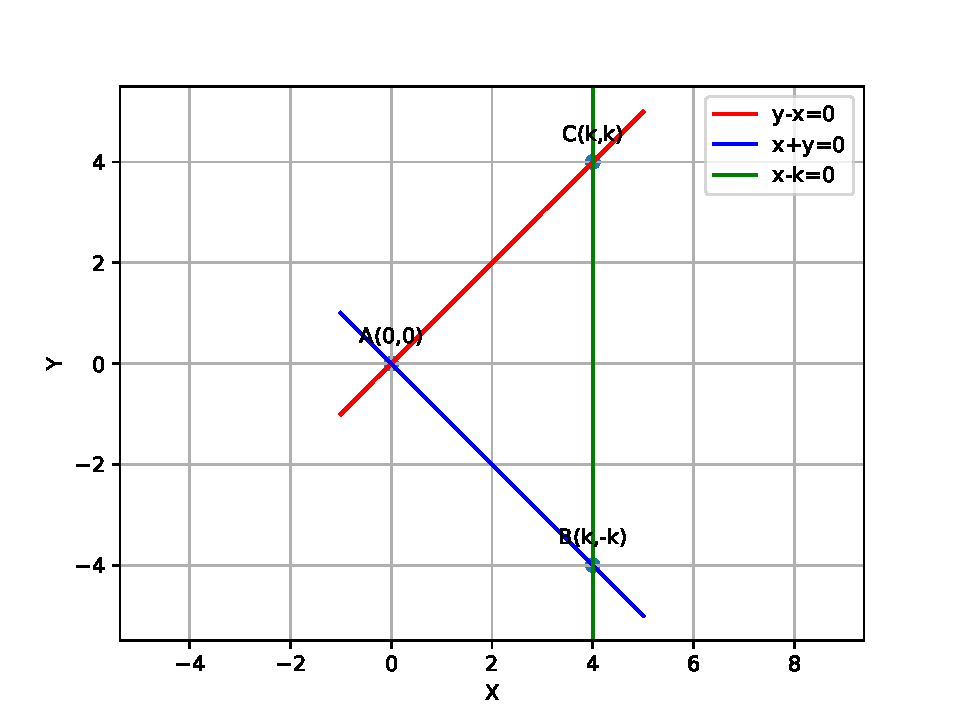
\includegraphics[width=\columnwidth]{./chapters/11/10/4/8/figs/fig.pdf}
	\end{center}
\caption{}
\label{fig:chapters/11/10/4/8/}
\end{figure}
